\section{Materials and Methods} \label{sec:methods}

\subsection{Avida Digital Evolution Platform}

\begin{figure}[!ht]
\centering
% https://docs.google.com/presentation/d/109vfeK_lHSsE0q7Iz7tzl9sDxnP8jyOF2gJ-v85pgL8/edit?usp=sharing
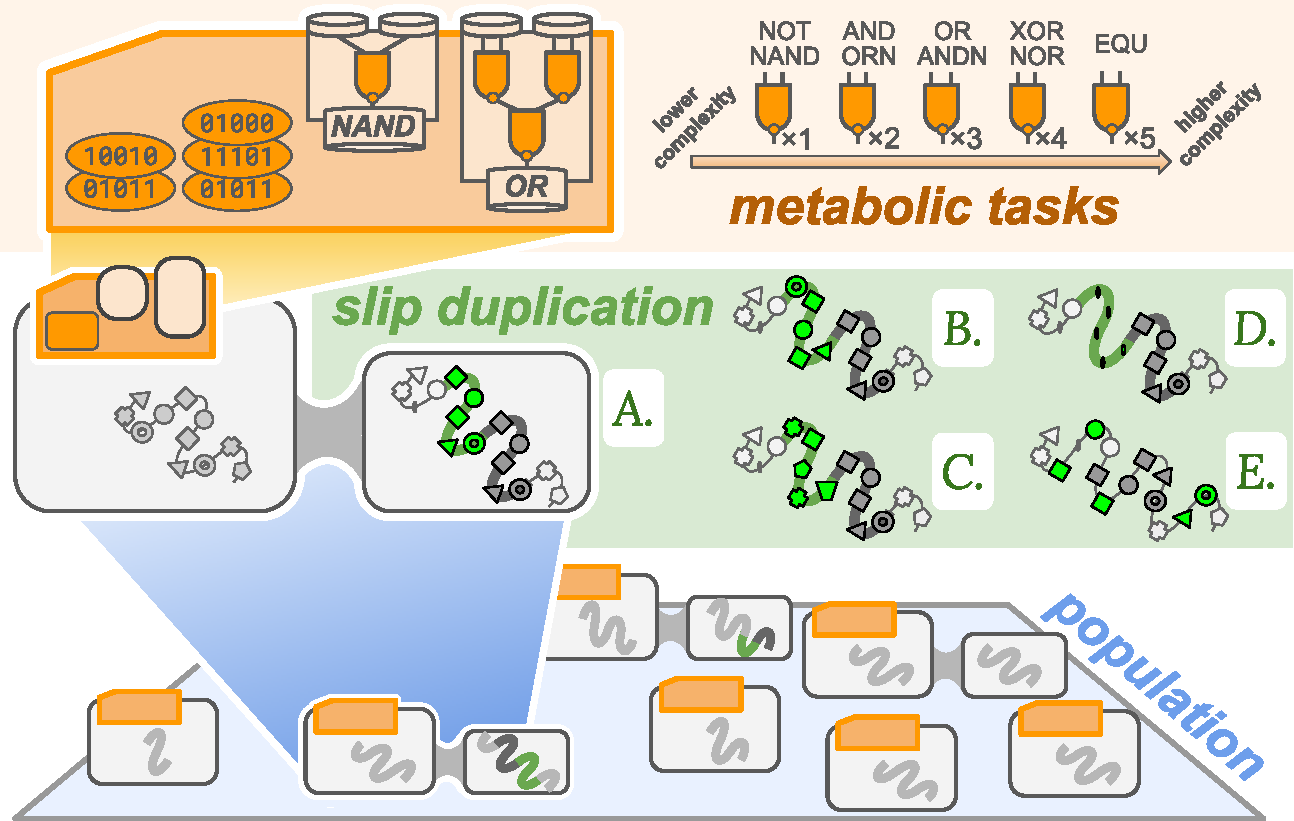
\includegraphics[width=\linewidth]{imgs/GeneDupeOps.pdf}

\vspace{2ex}

\caption{%
\textbf{Genome replication and phenotypic traits in Avida.}
\footnotesize
Self-replicating computer programs serve as digital model organisms (bottom panel).
Organisms comprise virtual stacks and registers used to store binary values and pointers within a genome of program instructions used to track instruction execution and copying.
Competition to survive and reproduce occurs within a limited-capacity population.
Replication activity can be accelerated by carrying out available ``metabolic'' input/output tasks (top panel).
These tasks vary in complexity with respect to the number of NAND operations required to perform them.
An organism's metabolic ``phenotype'' arises from the expression of its genetic code.
Genetic code copied from parent to offspring may be subject to point mutations, which change the individual instruction values, and slip mutations, which introduce or remove many instructions all at once (slip inserts shown as bright green).
Reported experiments compare five alternate variants of slip mutation:
A) \textit{Slip-duplicate}, an exact duplication is inserted adjacent to the target segment;
B) \textit{Slip-scramble}, shuffled duplication is inserted directly after the target segment;
C) \textit{Slip-random}, random instructions are inserted directly after the target segment;
D) \textit{Slip-NOP}, neutral nop-X instructions are inserted directly after the target segment; and
E) \textit{Slip-scatter}, randomly-drawn instructions are inserted at random throughout the genome.
}
\label{fig:slip_mut_variants}
\end{figure}


We conducted experiments using Avida, which instantiates an evolutionary process among self-replicating computer programs acting as ``digital organisms.''
This agent-based modeling approach allows research to empirically test hypotheses about evolution that would be difficult or impossible to test in natural systems \citep{Ofria:2009avida}.

% \begin{figure}[h]
   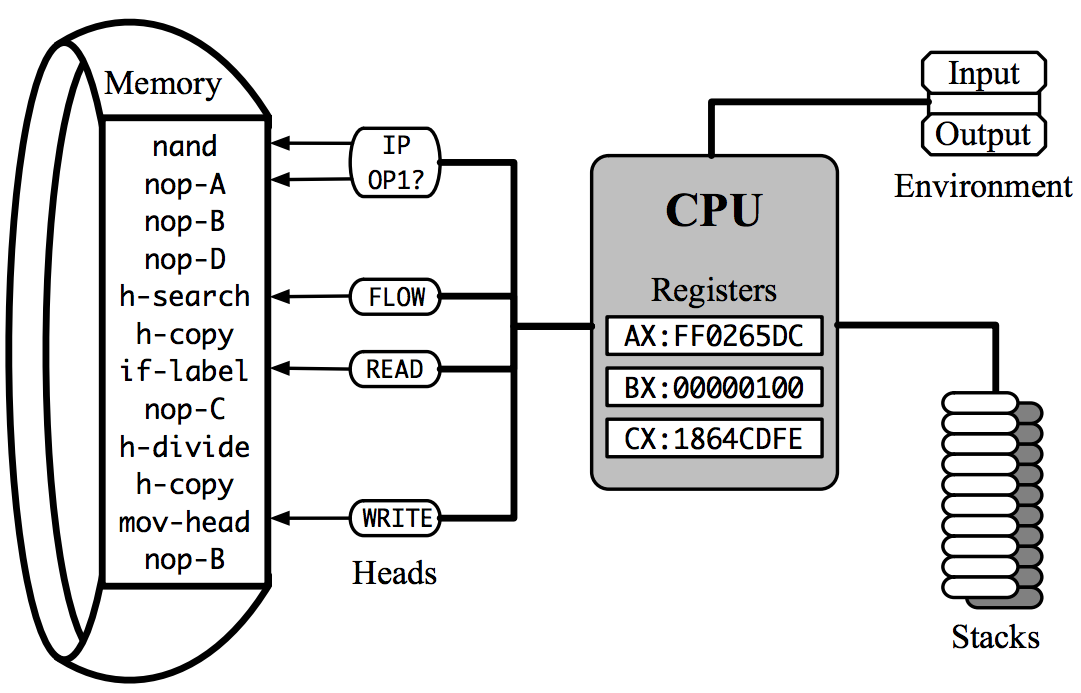
\includegraphics[width=\columnwidth]{imgs/virtual_hardware}
  \caption{\small Evaluation of Avida genome program instructions by virtual hardware, reproduced from \citep{Ofria:2009avida}.}
  \label{fig:vhardware}
\end{figure}


Digital organisms in Avida compete to acquire resources and replicate within a finite carrying capacity.
Each organism comprises a linear sequence of program instructions (\textit{i.e.,} its genotype), evaluated on an independent virtual processor.
The instruction set in Avida is Turing complete and syntactically robust, meaning that any ordering of instructions is syntactically valid.
The instruction set includes operations for basic computations, execution flow control, input and output, and self-replication.
% Figure \ref{fig:vhardware} overviews Avida virtual hardware used to evaluate program instructions.

Organisms in Avida replicate asexually by duplicating their genome one locus at a time.
Organisms' replication speed is influenced by their metabolic rate, which determines the speed at which they execute genome instructions.
At baseline, an organism's metabolic rate is set proportional to its genome length to prevent intrinsic disadvantages from increased copy loop duration for long genomes.
In our experiments, we increased metabolic rate for organisms exhibiting particular phenotypic traits, defined as output ``tasks'' requiring logical operations on input values.
In this way, we can define a set of discoverable adaptive phenotypic traits.

When an organism replicates, its offspring is placed at random elsewhere in the population, replacing any previous occupant of that location.
Thus, improving the efficiency of self-replication or performing rewarded computational tasks are both advantageous in the competition for space in Avida.
In combination with heritable variation introduced by program copy defects (discussed next), competition for population slots results in evolution by natural selection in Avida \citep{pennock2007models}.

Our simulations included four types of \textbf{mutational events in Avida}: substitution, insertion, deletion, or slip (duplication) mutations.

% https://github.com/chaynes2019/AvidaGeneDupe/blob/375f1a3018669f50d00e4ce67b977931cf42f6d9/experiments/2022-3-29-PaperDuplication/hpcc/config/avida.cfg
\textit{Copy mutations} introduce an erroneous \textit{substitution} where a random instruction is written into the offspring genome instead of the intended instruction.
In our experiments, such substitutions occurred with a per-copy probability of 0.0025.

\textit{Divide mutations} act on an organism's offspring during division.
When a divide \textit{insertion} mutation occurs, an arbitrary instruction is inserted at random, increasing the length of the offspring's genome by one.
When a divide \textit{deletion} mutation occurs, a random instruction in the offspring's genome is removed.
In our experiments, each was allowed to occur with a probability of 0.05 per offspring.

For the purposes of this study, we augmented Avida with a new type of divide mutation: \textit{slip mutation}.
This type of mutation acts analogously to gene duplications and deletions.
When a slip mutation occurs, two sites in the offspring genome are randomly selected, defining the target segment for the operation.
If the first site is upstream of the second, the slip mutation results in an insertion --- as if the organism's replication machinery had slipped backward during replication and copied a segment twice.
If the second site is upstream of the first, the slip mutation results in a deletion --- as if the organism's replication machinery skipped over a genetic segment.
As implemented, slip-insertions and slip-deletions occur with equal probability; thus, absent selection, this mutational process increases genome length variation but does not introduce an inherent bias on mean genome length.
% [x] @CAO: I limited this to a "directional" bias and made clear that it IS a dynamic to increase length variation.  Are we sure there won't be a directional bias on genome length?  It might be worth doing a simulated run (if it's quick) without any selection to control for any bias that might occur.  Think about it this way: as you get bigger, the average slip is bigger, but as you get smaller the average slip is smaller, so bigger genomes will change faster.  That said, if you are length 100 and have a slip of size 50, in on direction it changes your size to 0.5 what it was, but in the other it changes it by 1.5.  Frankly, I'm just not sure what would happen.
% @MAM good idea, did a quick random walk simulation and it looks like the mean value is stable https://gist.github.com/mmore500/92d2aee823b009319c47abab51e565cc

Across trials, we assessed full-fledged slip-duplicate mutation in comparison with four variant mutation operators with components disabled or replaced:
\begin{enumerate}
\item slip-scramble, where duplicated code was shuffled to test effects of sequence order,
\item slip-random, where duplicated code was replaced with random instructions to test effects of sequence content,
\item slip-NOP, where duplicated code was replaced with neutral (``no-operation'') instructions to test the effect of neutral increase in genome size, and
\item slip-scatter, where duplicated code was dispersed across the genome to test the effect of insertion locality.
\end{enumerate}
Figure \ref{fig:slip_mut_variants} provides an illustration of surveyed slip-mutation variants.
% [x] @CAO: I don't think it's worth starting whole new runs now, but the one other treatment I know we've at least talked about in the past is something like "slip-background" which is like slip-random, but where we look at the background distribution of instructions in the population to bias the random probabilities.  This can help distinguish why slip-scramble does better than slip random -- is it the instructions in the genome itself, or is it just that these are more likely to be instructions that are generally useful which is why they were selected by evolution in the first place.

When insertion occurs, all slip mutation operators add a number of instructions equal to the length of the target segment.
However, the composition and location of inserted instructions vary according to the slip mutation operator schema.
Deletions acted identically across slip mutation variants, except slip-scatter, which randomized deletions uniformly across the genome.
Where enabled, slip mutations occurred with 5\% probability per divide event.

\subsection{Experimental Design}

% \begin{table}[h]
\centering
\caption{Comlexity classifications of Logic-9 Boolean tasks. Reproduced from \citep{lenski2003evolutionary}.}
\label{tab:tasks}
\begin{tabular}{llc}
\hline
Task & Logic operation & \makecell{Complexity\\(num NANDs)} \\
\hline
NOT & $\sim$A; $\sim$B & 1 \\
NAND & $\sim$(A and B) & 1 \\
AND & A and B & 2 \\
OR\_N & (A or $\sim$B); ($\sim$A or B) & 2 \\
OR & A or B & 3 \\
AND\_N & (A and $\sim$B); ($\sim$A and B) & 3 \\
NOR & $\sim$A and $\sim$B & 4 \\
XOR & (A and $\sim$B) or ($\sim$A and B) & 4 \\
EQU & (A and B) or ($\sim$A and $\sim$B) & 5 \\
\hline
\end{tabular}
\end{table}


For our experiments, we configured available metabolic resources to the ``Logic-9'' task set, consisting of tasks NOT, NAND, OR-NOT, AND, OR, AND-NOT, NOR, XOR, and EQUALS.
Notably, the structure of this task set provides a well-defined difficulty gradient among tasks.
This characteristic arises from an explicit hierarchical composition among task definitions due to the fact that organisms only have direct access to the "Nand" instructions and must build all of the other tasks from different combinations of nands.
``Easier'' tasks like NOT and NAND form building blocks for ``more difficult'' tasks like XOR and EQU.
This well-defined gradient in task requirements provides a suitable apparatus for experiments involving the evolution of complexity \citep{lenski2003evolutionary}.
In this work, we categorize the complexity of the Logic-9 tasks by the minimal number of NAND building blocks\footnote{
In computer architecture theory, NAND is commonly established as the fundamental building block operation since all other logical operations can be derived from compositions of NAND gates \citep{mano1997logic}.
} required to perform them, as shown in Figure \ref{fig:slip_mut_variants}.
As such, we categorized tasks according to their NAND ``component counts'' as a proxy for phenotypic complexity.

Identical reward was provided for performing each task and kept consistent throughout trials.
Rewards were accrued independently for each task, allowing rewards to be compounded by performing multiple tasks.
We measured adaptation to the Logic-9 task set as a ``phenotypic adaptation score,'' ranging from a minimum of 0 (\textit{i.e.} the organism performs no tasks and received no reward) to a maximum of 9 (\textit{i.e.} the organism performs all 9 tasks and received the maximum reward).

Evolution experiments were conducted in two phases.
The first phase tested aggregate differences in evolutionary outcomes between surveyed slip duplication operator variants across runs, while the second focused more heavily on teasing apart evolutionary history and genetic structure within runs.
For this reason, first-phase experiments prioritized higher replicate counts, while second-phase experiments prioritized more detailed lineage tracking of individual genome sites.
Replicate count was 100 independent trials for first-phase experiments, and 30 replicates for second-phase experiments.
Run length was 200,000 updates across all experiments.
\footnote{An update in Avida is equal to the amount of time it takes for the average organism to execute 30 instructions; see \citep{Ofria:2009avida} for further detail.}
% Based on the timing of evolutionary convergence to stable states in the first phase experiments, a run length of 50,000 updates was used for second phase experiments.
This duration was sufficient to observe at least 600 generations of evolution in all trials.

Population size was configured to Avida default of 3,600 organisms across all trials.
Except where otherwise noted, experiments were seeded with a 100-instruction ancestral self-replicator.
In all cases, mutations reducing genome size below 100 instructions were disallowed to ensure sufficient raw genetic material to encode Logic-9 operations.

% % Color Definitions (for treatments table)
\newcommand\baselineratecolor{\cellcolor[HTML]{c9daf8}}
\newcommand\nonecolor{\cellcolor[HTML]{666666}}
\newcommand\slipdupcolor{\cellcolor[HTML]{4a86e8}}
\newcommand\slipscramcolor{\cellcolor[HTML]{8e7cc3}}
\newcommand\sliprandcolor{\cellcolor[HTML]{93c47d}}
\newcommand\slipnopcolor{\cellcolor[HTML]{ffd966}}
\newcommand\slipscattercolor{\cellcolor[HTML]{e06666}}
\newcommand\highmutcolor{\cellcolor[HTML]{ff9900}}

\begin{table*}[!ht]
  \centering
  \begin{tblr}{| c | c | c | c | c | c | c | c |}
    \hline
    \SetCell[r=2]{c} Treatment & \SetCell[c=2]{c} Slip Mutation & & \SetCell[r=2]{c} Substitution rate \\ per copy & \SetCell[r=2]{c} Insertion \\ and deletion rate \\ per copy & \SetCell[r=2]{c} Insertion and \\ deletion rate \\ per divide \\
    \cline{2-3}
    & Operator & Rate \\ per divide & & & \\
    \hline
    Baseline            & \nonecolor & \nonecolor & 0.0025 \baselineratecolor & \nonecolor & 0.05 \baselineratecolor  \\
    \hline
    Slip-duplicate      & Slip-duplicate \slipdupcolor & 0.05 \slipdupcolor   & 0.0025 \baselineratecolor & \nonecolor   & 0.05 \baselineratecolor  \\
    \hline
    Slip-scramble       & Slip-scramble \slipscramcolor & 0.05 \slipscramcolor    & 0.0025 \baselineratecolor & \nonecolor & 0.05 \baselineratecolor  \\
    \hline
    Slip-random         & Slip-random \sliprandcolor & 0.05 \sliprandcolor   & 0.0025 \baselineratecolor & \nonecolor & 0.05 \baselineratecolor  \\
    \hline
    Slip-NOP            & Slip-NOP \slipnopcolor  & 0.05 \slipnopcolor   & 0.0025 \baselineratecolor & \nonecolor & 0.05 \baselineratecolor  \\
    \hline
    Slip-scatter        & Slip-scatter \slipscattercolor & 0.05 \slipscattercolor & 0.0025 \baselineratecolor & \nonecolor & 0.05 \baselineratecolor  \\
    \hline
    High mutation rate  & \nonecolor & \nonecolor & 0.0025 \baselineratecolor & 0.0075 \highmutcolor & 0.05 \baselineratecolor \\
    \hline
  \end{tblr}
  \caption{\small Differences in mutation operators and rates among the seven treatments.}
  \label{table:treatments}
\end{table*}

First-phase experiments consisted of six treatments: one baseline treatment with slip-duplication disabled and five experimental treatments corresponding to the five surveyed slip-duplication mutation operators shown in Figure \ref{fig:slip_mut_variants}.
These treatments differed only in the available mutation operators and the rates at which those operators were applied.

% % Baseline treatment
% The \textbf{baseline treatment} was used as a control; we used the results from this treatment as a baseline for evolvability, with which we compared the results from all other experimental treatments. Mutation rates in the baseline treatment have been shown to facilitate both the evolution of complex boolean logic tasks, such as EQUALS, and the evolution of task regulation in Avida \citep{lenski2003evolutionary, Lalejini:2016plasticity}

% Long genome treatment
For second-phase experiments, we included an additional \textbf{long-genome baseline treatment} to directly test the adaptive role of large genome size associated with slip-duplicators.
Genomes in this treatment operated identically to those in the baseline treatment above, except that they were initialized with a 1,000-site ancestor.
We chose this size near the upper bound of genome sizes observed in first-phase slip-duplication treatment experiments.

% % Slip-duplicate treatment
% The \textbf{slip-duplicate treatment} allowed for mutation events that resulted in full code duplications via the slip-duplicate mutation operator. Duplications in this treatment preserved both the content and the structure of duplicated code. This allowed us to answer the following question: how important is it that gene duplications can exactly duplicate sequences in a genome in both content \textit{and} structure?

% % Slip-scramble treatment
% The \textbf{slip-scramble treatment} allowed for mutation events (via the slip-scramble operator) that resulted in code duplications where the content of the duplicated code was preserved, but the structure of the duplicated code was not preserved. This, compared with the slip-duplicate treatment, allowed us to answer the question: Is the duplication of particular instructions important, regardless of their arrangement?

% % Slip-random treatment
% The \textbf{slip-random treatment} allowed us to answer the following question: is it the case that gene duplications promote evolvability because they result in the insertion of large, clustered mutations, regardless of what those mutations may be? The slip-random treatment (via the slip-random mutation operator) allowed for mutation events that could insert large, contiguous clusters of random instructions; one could also think of these mutations as maximally noisy duplications where neither the content nor structure of the duplicated code is preserved.

% % Slip-NOP treatment
% The \textbf{slip-NOP treatment} allowed for mutations capable of inserting contiguous segments of blank `genetic tape' (via the slip-NOP mutation operator) in the form of no operation instructions. This allowed us to answer the following question: how important is it that gene duplications provide evolution with a straightforward technique for increasing genome size?

% % Slip-scatter treatment
% The \textbf{slip-scatter treatment} helped us tease apart whether gene duplications promote evolvability because they inflate the effective mutation rate, generating increased amounts of genetic variation. This treatment allowed for mutations that, when triggered, could insert many random instructions into random locations in a genome (via the slip-scatter mutation operator).

% In all experiments, organisms were limited to a minimum genome size (\textit{i.e.} instruction sequence length) of 100\footnote{
% In exploratory experiments, we found that, without enforcing a minimum genome size, slip mutations caused many lineages to quickly shrink in genome size because of inherent selection pressure for smaller genome size. Organisms became fast replicators but were then trapped on a local fitness optimum, unable to evolve to perform complex computational tasks.
% }.
% We limited the population size to 3600 and seeded each experiment with an ancestral genotype capable of self-replication, but no Logic-9 tasks.
% We ran between 30 and 100 trials of each treatment.

\subsection{Statistical Methods}

For first-phase experiments, we applied a Kruskal-Wallis test to screen for between-group variation in phenotypic adaptation score among surveyed treatments.
On account of an earlier experimental design incorporating two additional surveyed conditions incorporating environmental fluctuations, Bonferroni correction was applied to keep experiment-wise $\alpha$ = 0.05.
For subsequent Mann-Whitney U tests testing individual treatments against baseline, we applied Bonferroni correction for the five such comparisons.
Experimental design in our second-phase experiments did not require adjustments for multiple comparisons.

Time series assessments of evolutionary history were conducted using the ancestral lineage of the most abundant end-state genotype (``final dominant'').
In a postprocessing step, we applied Avida's ``analyze mode'' to identify each ancestor's tasks.
For investigations involving the evolutionary history of individual genome sites, we used mutational metadata saved with lineage files to identify corresponding sites between parent and offspring.
Due to memory constraints, these analyses were conducted from population save files recorded at update 50,000 rather than the end-state population at update 200,000.
This timepoint was chosen to encompass the phase in which the bulk of adaptive evolution had already transpired (see Figure \ref{fig:results_panels}).

\subsection{Software and Data Availability} \label{sec:materials}

Supporting software and executable notebooks for this work are available via GitHub at \url{https://github.com/chaynes2019/AvidaGeneDupe/} \citep{david_m_bryson_2025_14911296}.
Simulation data is archived via the Open Science Framework at \url{https://osf.io/j5s4h/} \citep{foster2017open}.

This project benefited significantly from a large number of open-source scientific software projects \citep{2020SciPy-NMeth,harris2020array,reback2020pandas,mckinney-proc-scipy-2010,waskom2021seaborn,hunter2007matplotlib,moreno2023teeplot,r_core_team_r:_2015}.
